% Diese Zeile bitte -nicht- aendern.
\documentclass[course=erap]{aspdoc}

%%%%%%%%%%%%%%%%%%%%%%%%%%%%%%%%%
%% TODO: Ersetzen Sie in den folgenden Zeilen die entsprechenden -Texte-
%% mit den richtigen Werten.
\newcommand{\theGroup}{196} % Beispiel: 42
\newcommand{\theNumber}{A328} % Beispiel: A123
\author{⁨Aleksandre Kandelaki \and Matthias Staritz \and Benjamin Liertz}
\date{Sommersemester 2020/21} % Beispiel: Wintersemester 2019/20
%%%%%%%%%%%%%%%%%%%%%%%%%%%%%%%%%

% Diese Zeile bitte -nicht- aendern.
\title{Gruppe \theGroup{} -- Abgabe zu Aufgabe \theNumber}

\begin{document}
\maketitle

\section{Einleitung}


Im Folgenden wird im Rahmen der Projektarbeit im Fach Einführung
in die Rechnerarchitektur an der TU München ein in linearer Algebra häufig 
benutztes Verfahren genauer beschrieben, implementiert und enstprechend dokumentiert.\\


Das Verfahren LU-Zerlegung, auch LR-Zerlegung genannt,
 bietet eine Möglichkeit per Algorithmus lineare Gleichungssysteme zu lösen und Matrixinverse zu bestimmen. 
 Dies Findet z.b. Anwendung bei der Berechnung des Stromflusses In Schaltkreisen. Mit der LU-Zerlegung kann man wenn man die Wiederstände einzelner Leitungen gegeben hat den Stromfluss an jedem Wiederstand berechnen. \cite{LUAnwendung}
Dazu liefert die LU-Zerlegung für jedes eindeutig
 lösbare Gleichungssystem, also wenn A regulär ist,
  zwei Dreiecksmatrizen L und U und eine Pivot-Matrix P,
   wobei P*L*U = A ergibt. Hierbei haben die Matrizen besondere 
   Eigenschaften. L hat in allen Einträgen oberhalb der Diagonalen die Werte 0 (Siehe Matrix \ref{unteremx}). U hingegen hat in allen Einträgen unterhalb
    der Diagonalen die Werte 0 (Siehe Matrix \ref{oberemx}). Die Matrix P ist eine Einheitsmatrix mit ggf. 
    vertauschten Zeilen (Siehe Matrix \ref{pivotmx}).
    \begin{equation}
\label{unteremx}
Untere Dreiecksatrix: \begin{bmatrix}

 x_{1,1}  & 0      &  0     & 0\\
 x_{2,1}  & x_{2,2}  &  0	  & 0 \\
 x_{3,1}	& x_{3,2}  & x_{3,3}  & 0\\
 x_{4,1}	& x_{4,2}	 & x_{4,3}  & x_{4,4} \\


 \end{bmatrix}
\end{equation}

\begin{equation}
\label{oberemx}
Obere Dreiecksatrix: \begin{bmatrix}
 x_{1,1}	& x_{1,2}	 & x_{1,3}  & x_{1,4} \\
 0	    & x_{2,2}	 & x_{2,3}  & x_{2,4}\\
 0	    & 0      & x_{3,3}  & x_{3,4}\\
 0	    & 0      & 0      & x_{4,4}\\
 \end{bmatrix}
\end{equation}

\begin{equation}
\label{pivotmx}
Pivotmatrix: \begin{bmatrix}

 x_{1,1}  & x_{1,2}	 & x_{1,3}  & x_{1,4} \\
 x_{2,1}  & x_{2,2}	 & x_{2,3}  & x_{2,4} \\
 x_{3,1}	& x_{3,2}  & x_{3,3}  & x_{3,4}\\
 x_{4,1}	& x_{4,2}	 & x_{4,3}  & x_{4,4} \\

\end{bmatrix}

\end{equation}


Ein anschauliches Beispiel hierzu wäre das lineare Gleichungssystem:
\begin{eqnarray}
0x_1 + 3x_2 + 5x_3 + 7x_4 = 0 \\
2x_1 + 6x_2 + 10x_3 + 14x_4 = 0\\
-4x_1 + 12x_2 + 15x_3 + -21x_4 = 0\\
6x_1 + 9x_2 + -5x_3 + -7x_4 = 0
\end{eqnarray}



Welches auch so dargestellt werden kann:
\begin{equation}
A = \begin{bmatrix}
 0	& 3	 & 5  & 7 \\
 2	& 6	 & 10 & 14 \\
-4	& 12 & 15 & -21\\
 6	& 9  & -5 & -7\\
 \end{bmatrix}
\end{equation}



Nach Anwendung der LU-Zerlegung ergeben sich folgende Matrizen:
 \begin{equation}

 A = \begin{bmatrix}
 0	& 3	 & 5  & 7 \\
 2	& 6	 & 10 & 14 \\
-4	& 12 & 15 & -21\\
 6	& 9  & -5 & -7\\
 \end{bmatrix}
  L =
 \begin{bmatrix}
 1	& 0	 & 0  & 0 \\
 0	& 1	 & 0 & 0 \\
-2	& 8 & 1 & 0\\
 3	& -3  & 4 & 1\\
 \end{bmatrix}
 U =
\begin{bmatrix}
 2	& 6	 & 10 & 14 \\
 0	& 3	 & 5 &  7 \\
 0	& 0  & -5 & -49\\
 0	& 0  & 0 &  168\\
 \end{bmatrix}
 P =
 \begin{bmatrix}
 0	& 1	 & 0 & 0 \\
 1	& 0	 & 0 & 0 \\
 0	& 0  & 1 & 0\\
 0	& 0  & 0 & 1\\
 \end{bmatrix}
 \end{equation}
 
 



\section{Lösungsansatz}
Zur Durchführung diser Zerlegung haben wir uns entschieden ein Programm auf Basis des gaußschen Eliminationsverfahren zu enwickeln.
Das gaußsche Eliminationsverfahren ändert die Einträge einer Matrix unter Verwendung elementarer Zeilenoperationen.
Die verwendeten elementaren Zeilenoperationen sind das Tauschen zweier Zeilen und das Addieren von
vielfachen einer Zeile auf eine Andere.
 Dabei wird das Gleichungssystem A*x = b verändert die Lösung bleibt aber erhalten.\\

Mit diesem Verfahren erstellen wir eine obere Dreieckmatrix bei der alle Einträge unter der 
Diagonalen 0 sind. So erhalten wir unsere U Matrix. Um nun auch unsere L und P Matrizen zu erhalten, müssen
wir nur alle Schritte die zur Generierung der U Matrix beigetragen haben Dokumentieren. Jedes mal wenn wir eine Zeile auf eine Andere addieren
wird dies in der L Matrix festgehalten indem genau die selbe Operation auf dieser L Matrix durchgeführt wird. Jede Zeilenvertauschung Wird auf die selbe Art in P festgehalten.  
Um nun sicher eine gültige L Matrix zu erhalten welche oberhalb der Diagonalen nur die 0 als Einträge hat und somit die gesuchte untere Dreiecksmatrix bildet, folgt der Algorithmus strikt der Vorgehensweise des Gauß Algorithmus.\\

Gehen wir davon aus das wir für jede der Matrizen L, U und P einen Speicherplatz haben.
Zu Beginn müssen die passenden Startwerte in diesen Matrizen abgelegt werden. In L und P sind das einfach Einheitsmatrizen und in U wird die Eingabematrix A geschriben. Nun Werden die Eintäge unterhalb der Diagonalen in U  
Spaltenweise von Links nach Rechts auf 0 gesetzt indem man immer ein genau passendes vielfaches einer oberen Zeile von allen darunterliegenden 
Zeilen abzieht. Die Wahl der Zeile hängt davon ab welche Spalte gerade auf 0 gesetzt werden soll. 
Bei Spalte 1 ist es Zeile 1 bei Spalte 2 Zeile 2 und so weiter. Da man sich hierbei von oben nach unten bwz. von links nach rechts Vorarbeitet generiert man schrittweise
die gewünschten L und U Matrizen. Nun kann es aber vorkommen dass in der Zeile welche von den anderen Zeilen subtrahiert werden soll an dem Index der zu bearbeitenden
Spalte eine 0 steht. Dies birgt das Problem dass nun kein vielfaches dieser Zeile jehmals die anderen Einträge der Spalte durch subtraktion auf 0 bringen kann
da $ 0 \times x = 0$. Um dieses Problem zu vermeiden haben wir uns entschieden generell, bevor wir mit der Nullung einer Zeile beginnen immer die Zeile mit dem größsten Eintrag
am entsprechenden Index nach oben zu Tauschen(Siehe Grafik). Dadurch wird Garantiert dass der Algorithmus bei einer regulären, quadratischen Matrix erfolgreich durchläuft. Im Abschnitt zur Genauigkeit wird noch genau darauf 
eingegeangen warum wir immer die Zeile mit dem größten Eintrag nach oben tauschen und nicht bloß Irgend eine Zeile mit Eintrag ungleich 0.
Zusätzlich sei gesagt dass nicht jede Matrixzerlegung den Schritt der Zeilenvertauschung benötigt und das der Algorithmus auf diese Art oft unnötige Vertauschungen durchführt was potential für 
Optimierungen bieten könnte.\\
 



\subsection{Stack vs. Heap}
 Bei der Wahl des Speicherortes muss noch eine weitere Gegebenheit beachtet werden.
 Undzwar haben wir hier die Wahl zwischen dem Heap und dem Stack. Auf Grund der besseren Zugriffszeiten des Stacks würden wir den Stack als Speicherort präferieren\cite{stack}.
 Aber leider wird bei Linux Betriebssystemen meistens blos circa 8MB Speicherplatz fuer die Stackallokationen zur Verfuegung gestellt.\cite{stackSize} Dies birgt für uns das Problem dass, sofern der Stack als Speicher genutzt wird,
 es bei zu großen Matrizen zu einem Segmentation Fault kommen kann. Um trozdem die bessere Performance des Stacks nutzen zu können haben wir eine Fallunterscheidung Implementiert welche jeh nach größe der Matrix entscheidet
 ob eine Matrix noch auf dem Stack zerlegt werden kann oder ob der benötigte Specherplatz auf dem Heap alloziert werden muss.
 Die Maximalgröße einer Eingabematrix dessen Zerlegung Stack durchgeführt werden kann berechnen wir folgender maßen:
 Die größe unserer Eingabematrix A muss 4 mal alloziert werden da temporär A, L, U und P abgespeichert werdem müssen.
 Der in der Methode übergebene Parameter n ist die Anzahl Zeilen / Spalten unseren Matrix da unsere Matrizem immer quadratisch sein müssen. Dadurch ergibt sich eine Anzahl Einträge pro Matrix von $n * n $. 
 Jeder dieser Einträge ist in unserem Fall ein Floating Point Wert und somit 4 Bytes groß.
 Daraus ergibt sich die Formel \ref{size} Welche die benötigte Anzahl bytes in Abhängigkeit unserer Eingabegröße n Berechnet.
 
 \begin{equation}
 \label{size}
  bytes = 4*4*n*n
 \end{equation}
Dann folgt dass unser $n$ für eine Nutzung des Stacks  $n <= 707$  sein muss.\ref{maxsize}
 \begin{equation}
 \label{maxsize}
  4*4*n*n <= 8*10^6
 \end{equation}
 Um etwas Spielraum zu haben haben wir uns entschieden schon ab einem $n >= 700$ auf dem Heap zu allozieren.\\


\subsection{Verschiedene Implementierungen}
Wie eben schon erwähnt ist uns aufgefallen dass die LU Zerlegung vieler Matrizen auch noch gelöst werden kann wenn man die Pivotisierung weg lässt. In der Theorie könnte man dadurch einen Performancgewinn erbringen. 
Um dies zu überprüfen haben wir eine Vergleichsimplementierung erstellt welche Pivotisierungen nicht berücksichtigt. Diese kann dann natürlich nicht mehr jede Matrix zerlegen hat aber potential schneller zu sein.
  Ansonsten ist diese Implementierung Analog zu obigen Ansatz.
Jenen Ansatz haben wir dann auf 3 verschiedene Arten Implementiert. Einmal in einfachen C, einmal unter Verwendung von Intrinsics und einmal als direktes Assembler Programm.
 Auf die speziefischeren Unterschiede wird im Abschnitt \ref{Performanzanalyse} noch genauer eingegangen.


% TODO: Je nach Aufgabenstellung einen der Begriffe wählen
\section{Genauigkeit}
- 

\section{Performanzanalyse}
\label{Performanzanalyse}
Die Laufzeit berechnet sich über  $ \frac{1}{3}n^3 -\frac{1}{3} n $ und befindet sich somit in $O(n^3)$ \cite{LULaufzeit}
In unserer Performanceanalyse vergleichen wir folgende Implementierungen:\\
\begin{itemize}
\item Lineare C Implementierung ohne Compileroptimierung und mit Pivotisierung vs. Lineare C implementierung ohne Compileroptimierung und ohne Pivotisierung. 
\item Lineare C Implementierung ohne Compileroptimierung vs. C Implementierung mit Vektorisierung durch Intrinsics. 
\item Lineare C Implementierung mit Compileroptimierung -O3 vs. Assembler Implementierung mit SIMD Vektorisierung.
\end{itemize}
Die Ergebnisse der Vergleiche werden in den folgenden Unterkapiteln ausgeführt. \\
\\


\subsection{Pivotisierung vs. keine Pivotisierung}
Leider ist der Perfomace Gewinn wie man an Grafik* unschwer erkennen Kann wenn überhaut bloß maginal. Dies kann man vermutlich auf zwei grundlegende Effekte zurückführen. Erstens Verändert das weglasen der Pivotisierung nicht die
 arithmethische Laufzeit welche weiterhin in $O(n^3)$ liegt. Der einzige Gewinn ligt also darin dass pro Schleifendurchlauf etwas weniger Operationen ausgeführt werden müssen. Dies kann aber maximal einen linearen Speedup erbringen. 
 Dieser lineare Speedup ist aber ebenfalls nicht wirklich signifikant da, wie man mit einer Performance Analyse erkennt, die Pivotisierung so oder so nur einen sehr kleinen Prozentsatz der Laufzeit beansprucht. 
 
 Unter Betrachtung dieser Erkenntnis zusätzlich zu den Ergebnissen der Genauigkeitsanalyse sind wir zu dem Schluss gekommen das eine Implementierung ohne Pivotisierung keinen Vorteil und Signifikante Nachteile bringt und dieser
  Ansatz somit nicht weiter Verfolgt werden muss.

\subsection{Linear vs. Parallel durch Intrinsics}
Eine Performanzanalyse unserer Linearen C Implementierung mit perf tool hat ergeben, dass ein Großteil der Rechenzeit in einer bestimmten Schleife verbracht wird. Ausserdem zeigt perf tool uns das innerhalb der
 Schleife die meiste Zeit für mov Befehle aufgewandt wird dicht gefolgt von arithmetischen Operationen. Diese Befehle sind in unserem Kontext Teil von Zeilenoperationen auf eine Matrix. Dies bedeutet dass diese Operationen zu 
 großen Teilen Unabhänig voneinander sind. Also können wir diese Operationen rellativ einfach, unter Zuhilfenahme von C Intrinsics, Parallelisieren.
 Die Laufzeit der Implementierung in der wir diese teuren Operationen vektorisiert haben wird In Abbildung 1 mit der Laufzeit der unvektorisierten Implementierung verglichen. 

 \begin{figure}[h]
\label{fig:perf1}
\caption{C-linear vs. C-vektorisiert}
 \centering
 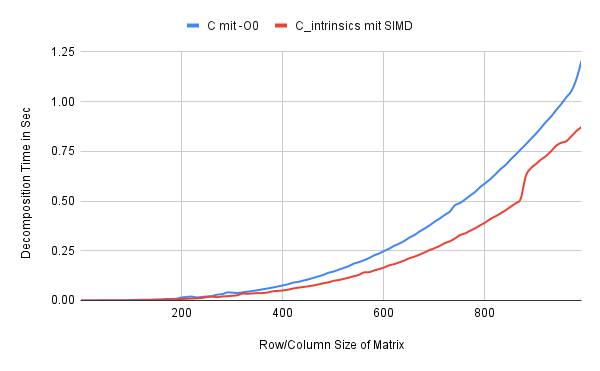
\includegraphics[width = 0.8\linewidth]{CvsIntrins.png}
 
\end{figure}
Durch den zusätzlichen Overhead der Vektorisieung sieht man bei kleineren Eingabegrößen keinen signifikanten Unterschied. Aber um so größer die Eingabe wird desto deutlicher sieht man, an den sich von einander entfernenden 
Graphen, dass die Vektorisierung einen guten Speedup generiert. 
Wir haben den Speedup Punktuell bei einer Eingabegröße von $n = 1000$ berechnet wo dieser bei ******** liegt.\\

 \subsection{Compiler optimierter Code vs. ASM mit SIMD}
Als letztes haben wir um optimale Performance zu erreichen eine reine ASM Implementierung entwickelt. In dieser Implementierung haben wir möglichst viel Optimiert und vor allem die im vorherigen Kapitel als Laufzeit aufwendig
 intendefizierten Stellen direkt mit xmm Instruktionen Vektorisiert. Zum Vergleich haben wir unsere einfache C Implementierung mit -O3 kompilliert um zu analysieren ob unsere Implementierung besser, schlechter oder ähnlich gut wie der Compiler ist.
 Wie man an Abbildung 2 erkennen kann bringt unsere händische Implementierung eine deutlich bessere Performance als die compileroptimierte Version. Dies Ist ein für uns überraschendes Ergebnis was uns aber zeigt das 
 es manchmal tatsächlich noch sinnvoll sein kann Assembler Code per Hand zu schreiben.

 \begin{figure}[h]
\label{fig:perf2}
\caption{C-ompileroptimiert vs. Assembler-vektorisiert}
 \centering
 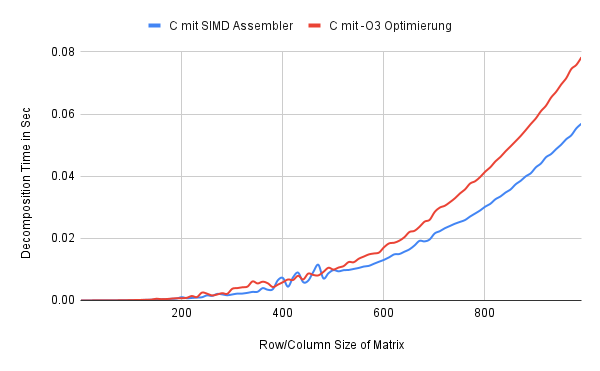
\includegraphics[width = 0.8\linewidth]{CvsASM.png}
 
\end{figure}



\section{Zusammenfassung und Ausblick}
Welche Performance war jetzt am besten?\\
Rückblickend hätte man ohne pivotisierung weglassen können\\
% TODO: Fuegen Sie Ihre Quellen der Datei Ausarbeitung.bib hinzu
% Referenzieren Sie diese dann mit \cite{
% Beispiel: CR2 ist ein Register der x86-Architektur~\cite{intel2017man}.
\bibliographystyle{plain}
\bibliography{Ausarbeitung}{}

\end{document}

